\subsection{Level3.1: パラメータのチューニング}%
\subsubsection{最適なパラメータを探すためのアプローチ}
指定された条件下において学習が効率良く行われるパラメータの組み合わせを探
すため、
hiddenを10から100まで10づつ増やしていき,etaを0.01から1.98まで0.01づつ増
やし,alphaを0.1から1.0まで0.1づつ増やしていきその中から一番値が小さい物
を探した.その動作をスクリプトを書いて実行させた.

\subsubsection{実行結果}
各パラメータが T A 1.7126, ALPHA = 694, HIDDEN 3016 の時, 3 のよ
うな結果が得られた.その時の学習曲線 は図43 のようになる.
\begin{table}[htb]
 \begin{center}
  \caption{階層型NNによる文字認識問題の学習に要した回数}
  \label{table:level3}
  \begin{tabular}[htb]{r|l} \hline
   シード値 & 収束した回数 \\ \hline \hline
   1000 & 97 \\ \hline
   2000 & 81 \\ \hline
   3000 & 108 \\ \hline
   4000 & 106 \\ \hline
   5000 & 46 \\ \hline
   6000 & 130 \\ \hline
   7000 & 85 \\ \hline
   8000 & 89 \\ \hline
   9000 & 134 \\ \hline
   10000 & 84 \\ \hline \hline
   10試行の平均値 & 95.9 \\ \hline
  \end{tabular}
 \end{center}
\end{table}

\begin{figure}[h]
 \begin{center}
  \includegraphics[width=10.0cm]{ave.eps}
  \caption{重みを更新する様子(平均値)}
  \label{fig:level2}
 \end{center}
\end{figure}
\newpage


